\begin{quote}
	``Most tasks that consist of mapping an	input vector to an output vector, and that are \emph{easy for a person to do rapidly}, can	be accomplished via deep learning, given sufficiently large models and sufficiently	large datasets of labeled training examples.''\cite[p.\,167]{Goodfellow-et-al-2016}
\end{quote}

Although being more of an intuition than a formal rule, above quotation might capture the reason for this work's failure. Even after simplification of the problem or after increasing the amount of training data, the network always failed to beat the simplest prediction even a human could do: To assume the next day's prices are identical to today.
Referencing section~\ref{sec:deep-learning} at the beginning of this work, even though a neural network can learn any such function, it might just learn the most obvious one.

To explore the neural network's approach to learning, one might look at an even simpler task for this work's problem: Instead predicting prices (i.e. real values) the network gets to decide a range of the next day's prices. Therefore going from a regression to a classification task.

\section{Digression: Classification approach}

The network's architecture is mostly the same as for regression. There are some differences in the choice of loss function and for some activations, but in general the network should predict if the next day's spread price is above $0.1$, below $-0.1$ or in between, resulting in three classes. The network's performance is captured by calculating its accuracy: the ratio of correctly classified samples to their total number.

Training six networks -- one for each leg of the spread prices' term structure, each with depth $1$ and width $30$ -- results in the accuracies shown in~figure~\ref{fig:classification-results}. A higher accuracy is equivalent to a better performance.
The results are quite familiar: Again, the network performs slightly worse than a native prediction (a). Even though the task is much simpler, the learned mapping is far from sophisticated. By predicting farther into the future (b) there is some interesting detail: Again the networks' performance follows the naive prediction with some gap. But at around $0.5$ accuracy the network's predictions stabilize because there seems to be a promising strategy (but surely of similar simplicity) than just approximating a naive prediction or randomly guessing. Nevertheless, this accuracy is far from satisfactory and does not justify the usage of neural networks.

\begin{figure}
	\centering
	\begin{subfigure}{0.49\linewidth}
		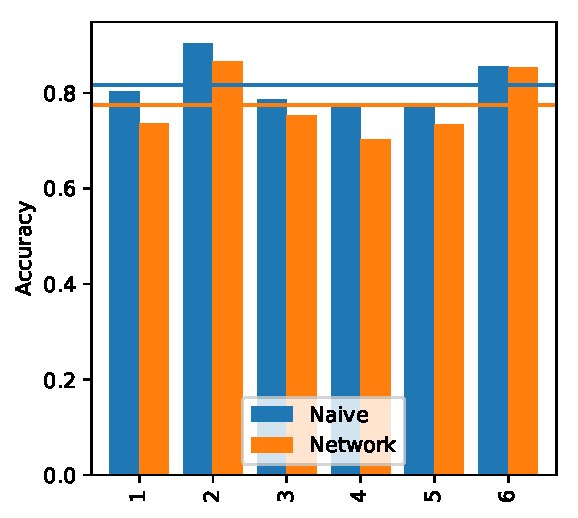
\includegraphics[width=\linewidth]{classification-1}
		\caption{}
	\end{subfigure}
	\begin{subfigure}{0.49\linewidth}
		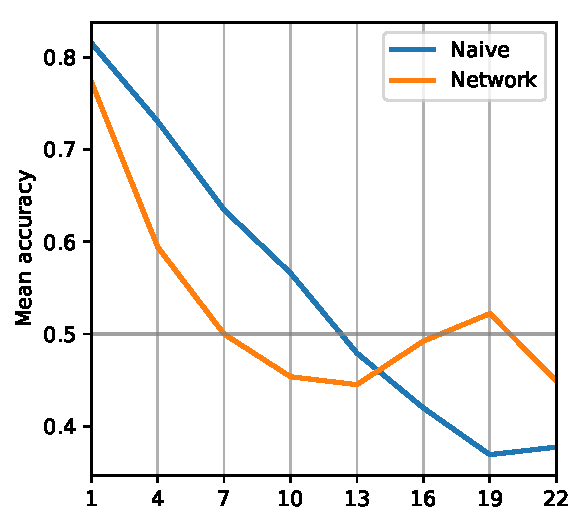
\includegraphics[width=\linewidth]{classification-all}
		\caption{}
	\end{subfigure}
	\caption[Results of classification approach]{Results of classification approach using a network with depth $L=1$, width $K=1$ and three classes. The performance measure is classification accuracy, meaning higher values are better. (a) Legwise accuracy for predicting the next day. (b) Mean accuracy over all legs for predicting up to 22 days into the future.}
	\label{fig:classification-results}
\end{figure}

\section{Lookout}

The most impressive results of artificial neural networks are in areas humans are originally good at: vision, language and speech. This work was about exploring a task even humans have problems with: Financial analysis and prediction. 

Showing the shortcomings of neural networks, does this mean deep learning is useless in finance? I believe not. Finance is a vast field and because of such networks' ability to process large amounts of data and to find non-linear patterns for a possible huge number of inputs there are surely many sensible applications. Even if many of these patterns could be recognized by humans, the sheer amount of information might deem neural networks suitable. For some inspirations see \cite{DBLP:journals/corr/HeatonPW16} or \cite{Mao-2011}.
Furthermore there exist many other successful techniques -- some of classical background, some from the area of machine learning -- for different kinds of problems. A recent comparison was made in \cite{DBLP:journals/corr/QianG17}. It is choosing the right tool for the right job.

For future use of deep learning on similar problems one might consider using a much larger number of inputs. Also, \emph{self-normalizing neural networks} as shortly presented in section~\ref{sec:hyperparameters} seem to be a promising approach, provided the data satisfies the mathematical properties necessary. But most of all one needs to reconsider the end-to-end approach of deep learning like applied in other areas. Its potential in finance might be more as one part of a larger pipeline, seeing it just as one method out of many.